\chapter{Các công trình liên quan}
\label{Chapter2}

Bài toán sinh cử chỉ là cũng tương tự như các bài toán khác đều đã nghiên cứu và phát triển song hành cùng các phương pháp học máy truyền thống cũng như các phương pháp học sâu hiện đại ngày nay, gồm các nhóm phương pháp dựa trên luật và các phương pháp dựa trên dữ liệu. 

\section{Mối quan hệ giữa cử chỉ và lời nói}

Cử chỉ được chia thành 6 nhóm chính theo ngôn ngữ  học \cite{ekman1969repertoire}, \cite{sebeok2011advances} cử chỉ thích nghi (adaptors), cử chỉ biểu tượng (emblems), cử chỉ chỉ định (deictics), cử chỉ biểu trưng (iconics), cử chỉ ẩn dụ (metaphorics) và cử chỉ nhấn mạnh (beat).

 Trong đó, cử chỉ nhấn mạnh không liên quan trực tiếp đến ngữ nghĩa lời nói \cite{kipp2005gesture} nhưng rất quan trọng để tạo sự hài hòa về nhịp điệu giữa lời nói và cử chỉ  \cite{sebeok2011advances} . Tuy nhiên, lời nói và cử chỉ nhấn mạnh không đồng bộ hoàn toàn về mặt nhịp điệu \cite{mcclave1994gestural}, nên việc học mối liên hệ thời gian giữa chúng gặp khó khăn \cite{bhattacharya2021speech2affectivegestures}, \cite{kucherenko2020gesticulator}, \cite{yoon2020speech}.

Cử chỉ liên quan đến các cấp độ khác nhau của thông tin lời nói \cite{sebeok2011advances}. Ví dụ, cử chỉ biểu tượng như cầm ngược cái ngón cái thường đi kèm với ngữ nghĩa cấp cao như tốt hay tuyệt vời, trong khi cử chỉ nhấn mạnh thường xuất hiện cùng với sự nhấn mạnh âm thanh cấp thấp. Nhiều nghiên cứu trước đây chỉ sử dụng các đặc trưng được trích xuất từ lớp cuối cùng của bộ mã hóa âm thanh để tổng hợp cử chỉ \cite{alexanderson2020style},  \cite{bhattacharya2021speech2affectivegestures}, \cite{kucherenko2021large}, \cite{qian2021speech},  \cite{yoon2022genea}. Tuy nhiên, cách thiết lập này có thể khuyến khích bộ mã hóa trộn lẫn thông tin lời nói ở nhiều cấp độ khác nhau vào cùng một đặc trưng, gây ra sự mơ hồ và tăng độ khó khăn trong việc khai thác các dấu hiệu nhịp điệu và ngữ nghĩa rõ ràng.

%Trong bài báo này, chúng tôi tập trung vào việc tạo ra cử chỉ trên đi kèm lời nói có thể đồng hành với một loạt các nội dung lời nói rộng - từ một câu đến bài phát biểu công khai, nhằm đạt được kết quả thuyết phục cả về nhịp điệu và ngữ nghĩa. Quan sát đầu tiên của chúng tôi là cử chỉ có thể được coi là một dạng nhảy đặc biệt dưới nhịp điệu thay đổi. Chúng tôi phát triển một khuôn khổ chuẩn hóa và tạo ra nhịp điệu để đối phó với thách thức tạo ra cử chỉ đồng bộ với lời nói, phân đoạn lời nói thành các đoạn ngắn tại các nhịp âm thanh, chuẩn hóa các đoạn này thành các khối chuẩn có cùng độ dài, tạo ra cử chỉ cho mỗi khối và căn chỉnh chuyển động được tạo ra với nhịp điệu của lời nói. Khuôn khổ này, được lấy cảm hứng một phần từ các nghiên cứu gần đây về tạo múa \cite{aristidou2022rhythm}, cung cấp cho mô hình cử chỉ một gợi ý rõ ràng về nhịp điệu, cho phép mô hình học hiệu quả mẫu cử chỉ nhấn mạnh trong một khối nhịp điệu. 
%Cả đánh giá định lượng với một chỉ số nhịp điệu mới và đánh giá chất lượng với nghiên cứu người dùng đều cho thấy cử chỉ được tạo ra bởi quy trình này thể hiện sự đồng bộ tự nhiên với lời nói.

Như được chỉ ra trong các tài liệu ngôn ngữ học \cite{kipp2005gesture} \cite{neff2008gesture} \cite{webb1997linguistic},
cử chỉ được sử dụng trong cuộc hội thoại hàng ngày có thể được chia thành một số lượng hạn chế các đơn vị ngữ nghĩa với các biến thể chuyển động khác nhau. Chúng tôi giả định rằng các đơn vị ngữ nghĩa này, thường được gọi là từ ngữ, liên quan đến các đặc trưng cấp cao của âm thanh lời nói, trong khi các biến thể chuyển động được xác định bởi các đặc trưng âm thanh cấp thấp. Do đó, chúng tôi tách rời các đặc trưng cấp cao và cấp thấp từ các lớp khác nhau của bộ mã hóa âm thanh và học các ánh xạ giữa chúng và các từ ngữ cử chỉ và các biến thể chuyển động, tương ứng. Các thử nghiệm chứng minh cơ chế này thành công trong việc tách rời các đặc trưng ở nhiều cấp độ của cả lời nói và chuyển động và tổng hợp các cử chỉ phù hợp về mặt ngữ nghĩa và có phong cách.

\section{Tổng quan các phương pháp cho bài toán sinh cử chỉ}

\subsection{Phương pháp dựa trên luật}

Các phương pháp dựa trên luật thường ánh xạ (mappings) từng âm thanh với từng đơn vị cử chỉ \cite{huang2012robot}. Và luật được tạo thủ công. Phương pháp dựa trên luật thì chúng ta có thể dễ dàng điều khiển kết quả của mô hình và có khả năng giải thích tốt kết quả dự đoán của mô hình.
Tuy nhiên chi phí để tạo thủ công là không khả thi để xây dựng cho các ứng dụng phức tạp đòi hỏi phải xử lý một lượng dữ liệu rất lớn.

\subsection{Phương pháp dựa trên thống kê}

Tương tự như phương pháp dựa trên luật, phương pháp dựa trên dữ liệu cũng ánh xạ các đặc trưng của âm thanh tương ứng với cử chỉ nhưng thay vì làm thủ công thì được sử dụng học một cách tự động dựa trên dữ liệu.
Trong đó có hai phương pháp chính là phương pháp thống kê và phương pháp dựa trên dữ liệu.

%\subsubsection{Phương pháp thống kê}

Phương pháp thống kê sử dụng phân phối xác xuất để tìm sự tương đồng giữa các đặc trưng âm thanh và cử chỉ \cite{levine2010gesture}. Tác giả \cite{neff2008gesture} xây dựng mô hình để học từng phong cách của từng người nói.

\subsection{Phương pháp học sâu}

\setcounter{figure}{3}
\begin{figure}
	\centering
	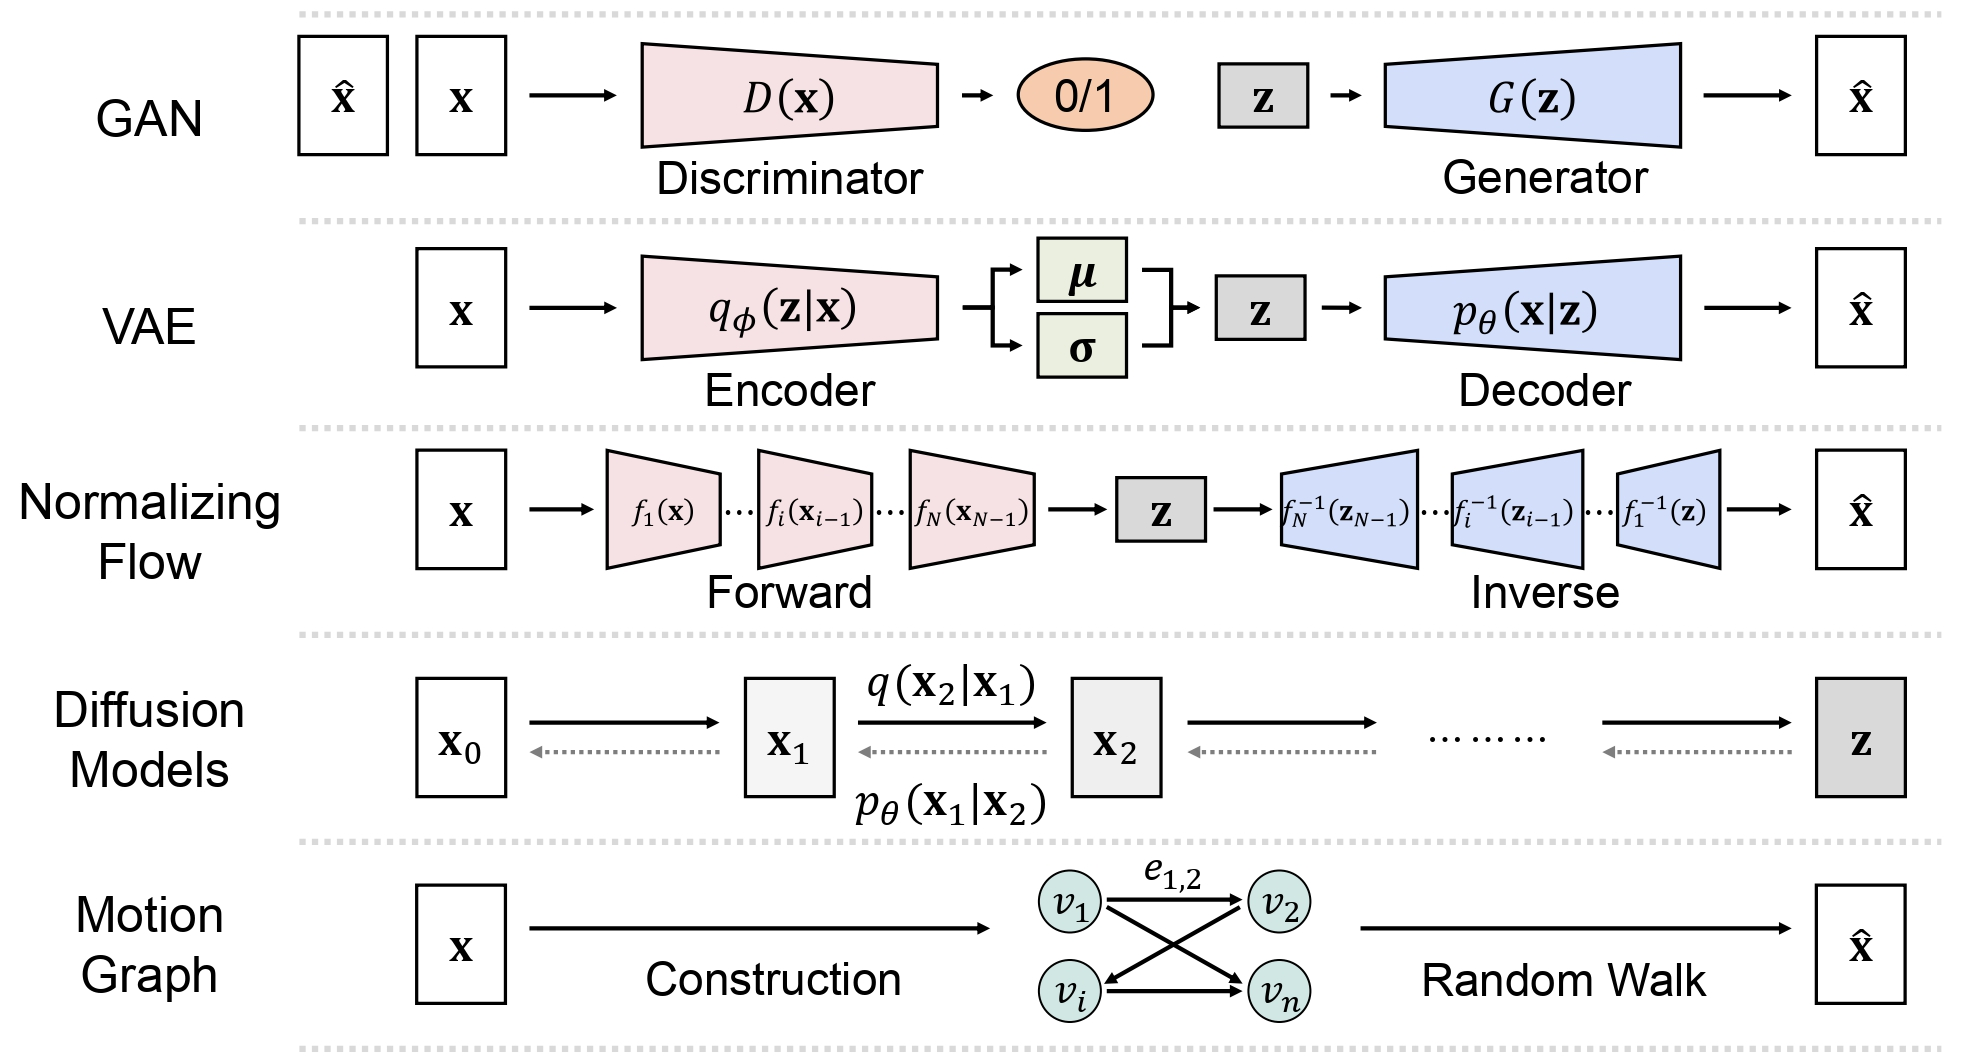
\includegraphics[width=0.8\textwidth]{Survey.jpg}
	\caption{Tổng quan về các mô hình tạo sinh khác nhau.}
	\label{fig:generative-models}
\end{figure}

Phương pháp sinh cử chỉ được chia thành hai nhóm chính. Bao gồm các mô hình ước lượng log likelihood (likelihood-base model)  và phương pháp dựa vào các mô hình sinh ngầm định (implicit generative models).

\subsubsection{Likelihood-base Model}

Phương pháp học ước lượng log likelihood là phương pháp học trực tiếp từ hàm mật độ xác xuất (probability density) thông qua maximum likelihood. Các phương pháp điển hình là autoregressive models, normalizing flow models, energy-based models (EBMs)
, và variational auto-encoders (VAEs).

%Phương pháp học sâu sử dụng mạng nơ-ron (neural) thông qua nhiều lớp ẩn để học một cách tự động các phối xác xuất giữa cử chỉ và âm thanh.

Mô hình được kết hợp với văn bản đầu vào được gắn thẻ với chủ đề, trọng tâm câu và thành ngữ để tạo ra các kịch bản cử chỉ, sau đó được ánh xạ sang một chuỗi các cử chỉ được chọn từ một từ điển hoạt họa. \cite{chiu2015predicting} huấn luyện một model classifier neuron network để chọn một đơn vị cử chỉ phù hợp dựa trên đầu vào là lời nói. 
%Nghiên cứu gần đây đã bắt đầu tận dụng học sâu và huấn luyện các mô hình kết thúc đến cuối sử dụng dữ liệu cử chỉ thô trực tiếp, giải phóng các nỗ lực thủ công trong thiết kế từ điển cử chỉ và các quy tắc ánh xạ.

Cử chỉ có thể được tổng hợp bằng các mô hình xác định như perceptron đa tầng (MLP) \cite{kucherenko2020gesticulator}, recurrent neural networks \cite{bhattacharya2021speech2affectivegestures}, \cite{liu2022learning}, \cite{hasegawa2018evaluation}, \cite{yoon2020speech}, convolutional networks \cite{habibie2021learning} và transformer \cite{bhattacharya2021text2gestures} 

%và các mô hình như normalizing flow \cite{alexanderson2020style}, 
%phương pháp học code  \cite{xu2022freeform}.

\subsubsection{Implicit Generative Models}

Trong các phương pháp dựa vào mô hình sinh ngầm định, phân phối của dữ liệu được học một cách ngầm định thông qua việc quá sinh lấy mẫu (sampling). Ví dụ tiêu biểu nhất là mô hình generative adversarial networks (GANs). Khi dữ liệu được tổng hợp bằng cách chuyển phân phối dữ liệu ban đầu ở dạng phân phối chuẩn về phân phối của dữ liệu.

Trong mục tiêu theo chúng tôi sẽ trình bày các phương pháp sử dụng mô hình Diffusion.

%chuyển phân phối của dữ liệu ở dạng phân phối chuẩn hay ở một vị trí bất kỳ về phân phối chuẩn bằng hàm neuron network. 


%WGAN \cite{wu2021probabilistic}.



%\textbf{Bảng so sánh các phương pháp}
%
%\begin{table}[ht]
%	\centering
%	\begin{tabular}{|l|l|l|l|l|l|}
%		\hline
%		\textbf{Phương pháp} & \textbf{Loại mô hình} & \textbf{Đặc điểm nổi bật} & \textbf{Ưu điểm} & \textbf{Hạn chế} & \textbf{Tài liệu tham khảo} \\ \hline
%		VAE  & Autoencoder & Biểu diễn dữ liệu trong không gian tiềm ẩn & Tạo đặc trưng ẩn & Khó kiểm soát đầu ra & \cite{kingma2013auto} \\ \hline
%		VQ-VAE & Autoencoder (cải tiến) & Dùng codebook cho không gian tiềm ẩn & Biểu diễn chi tiết hơn & Phức tạp hơn & \cite{van2017neural} \\ \hline
%		RNN & Mạng hồi tiếp & Xử lý chuỗi dữ liệu & Tốt cho dữ liệu tuần tự & Khó huấn luyện & \cite{bhattacharya2021speech2affectivegestures} \\ \hline
%		Transformer & Mạng chú ý & Tạo cử chỉ qua cơ chế chú ý & Hiệu quả với dữ liệu dài & Yêu cầu nhiều tài nguyên & \cite{bhattacharya2021text2gestures} \\ \hline
%		WGAN & GAN & Học phân phối dữ liệu đối kháng & Tạo sự đa dạng & Khó huấn luyện & \cite{wu2021probabilistic} \\ \hline
%		Normalizing Flow & Mô hình xác suất & Học phân phối phức tạp & Hữu ích với dữ liệu phức tạp & Cần tài nguyên tính toán lớn & \cite{alexanderson2020style} \\ \hline
%		Diffusion Models & Mô hình sinh dữ liệu & Chi tiết cao, xử lý dữ liệu thiếu & Tạo cử chỉ chi tiết & Thời gian huấn luyện lâu & \cite{xu2022freeform} \\ \hline
%	\end{tabular}
%	\caption{So sánh các phương pháp sinh cử chỉ}
%\end{table}

%